%------------------------------------------------------------------------------
% This is a LaTeX template for the scientific justification of IRAM Proposals 
%------------------------------------------------------------------------------
% 
% We encourage IRAM proposers to use this template for the sake of unity 
% and clarity when Program Committee members assess their proposals.
% 
% You may customize this template to suit your preferences (e.g. using BibTex),
% but please respect the following requirements:
%     The scientific justification should contain a maximum of 2 pages of text 
%     (4 pages for Large Programs), plus 2 pages of Figs., Tables and Refs.
%     The font size should be 11pt or larger.
%
% For Large Programs, the following sections should be included: 
%   i) Scientific Rationale, 
%  ii) Immediate Objective, 
% iii) Feasibility and Technical Justification, and 
%  iv) Organizational Issues.
% 
%
%------------------------------------------------------------------------------
%
\documentclass[11pt,a4paper,twoside,graphicx,color]{article}
%
\usepackage[margin=2cm]{geometry}
\usepackage[pdftex]{graphicx}
\usepackage{color}
\usepackage{txfonts}
\usepackage{paralist}
\usepackage[numbers]{natbib}
\setlength{\bibsep}{0.0pt}
\usepackage{amssymb}

\newcommand{\ccor}[1]{\textcolor{red}{#1}}

%
% Page size and text dimensions
% Do not change!
\textheight 260mm
\textwidth 178mm
\oddsidemargin -8mm
\evensidemargin -8mm
\marginparwidth 50pt
\topmargin -22mm
\brokenpenalty=10000
\sloppy
%
%-------------------------------------------------------------------
\begin{document}
\def\moo{MOO\,J1142$+$1527}
%
%
\begin{center}{\huge \bf
%-------------------------------------------------------------------
High resolution SZ observations of the massive and distant cluster \moo\ with NIKA2
%-------------------------------------------------------------------
}\end{center}
% 
\centerline{\bf P.I.: B. Comis \& F. Ruppin}

\section{Scientific context}
{\bf \large Introduction -- } 
Galaxy clusters are the ultimate manifestation of the hierarchical structure formation process in the standard cosmological model, and as such, they are sensitive to both the matter content and expansion history of the Universe in which they form. Clusters of galaxies are thus powerful tools to characterize the \textbf{formation processes of large scale structures}. Although hierarchical gravitational collapse of small structures seems to be the main driver of cluster formation, non-gravitational processes such as feedback from AGN and supernova-driven galactic winds may alter cluster observables to a large extent. Consequently a detailed characterization of the complex interplay between gravitational and non-gravitational processes acting on clusters is mandatory for \textbf{a detailed understanding of their astrophysics}.

The principal baryonic component of galaxy clusters is found in the hot, ionized, X-ray emitting gas of the intracluster medium (ICM), containing about 12\% of the total mass. Cluster thermodynamics and dynamical properties can be inferred from several independent observables. The velocity dispersion of the galaxies \cite{sif16}, various X-ray properties such as temperature or luminosity \cite{pra09}, or the lensing distortions of background galaxies \cite{hoe15} can be related to the underlying total mass. Another observational probe of interest is \textbf{the thermal Sunyaev-Zel'dovich effect} (tSZ) \cite{sun72} which is due to the inverse Compton scattering of cosmic microwave background (CMB) photons with high energy electrons of the ICM. As this effect is directly proportional to the thermal energy contained in the ICM, it is expected to provide a low scatter mass proxy for galaxy clusters \cite{nag07}. Furthermore, as the tSZ effect is a CMB spectral distortion, it does not suffer from cosmological dimming. This observable is therefore a powerful probe to estimate both galaxy cluster total mass and baryonic content distribution \textbf{up to very high redshift}.

\textbf{The high mass tail} of the galaxy cluster population is of significant interest for both galaxy evolution and cosmology. For cosmology, massive, high-redshift clusters remain competitive probes of dark energy via a number of methods, including evolution in the cluster mass function \cite{vik09}, the clustering of galaxy clusters \cite{ser15}, and through application of the $f_{gaz}$ test \cite{man14}. The high mass tail of the galaxy cluster mass function is also a sensitive indicator of primordial non-Gaussianity \cite{sha13}.

In the last several years, the SZ dedicated instruments SPT, ACT and Planck have each completed wide-area millimeter surveys to identify galaxy clusters via the Sunyaev-Zel’dovich effect, finding about \textbf{50 massive clusters at $\mathbf{z > 1}$}. However, the \textbf{upcoming generation of optical, galaxy-based cluster searches will also extend into the wide-area, high-redshift region of parameter space}, complementing these millimeter surveys. 

\textbf{The Massive and Distant Clusters of WISE Survey} (MaDCoWS), designed to detect the most massive galaxy clusters at $z \sim 1$, offers the largest survey area among current high-redshift cluster searches. It uses infrared WISE and PanSTARRS optical imaging to robustly isolate galaxy clusters at $z \sim 1$ over more than 80\% of the extragalactic sky. The first phase of MaDCoWS
covered $\sim 10,000~\mathrm{deg}^2$ within the SDSS footprint; subsequent phases of the program are now extending the search over the full extragalactic sky.

In the coming years such optical surveys will provide interesting cluster samples for the high-mass and high-redshift population. And these will of course represent further interesting targets for the NIKA2 camera and SZ science. Combining the sub-arcminute resolution NIKA2 SZ data with the Planck view of such clusters, we will also explore the possible impact and future perspectives of combining the complementarity of these two SZ instruments for the so called " pink elephants ".

\noindent {\bf \large Previous observations with NIKA -- } 
The NIKA prototype has been used as a pathfinder for NIKA2, to demonstrate the possibility to use large arrays of Kinetic Inductance Detectors (KIDs) in millimeter astronomy and to validate the observation strategy as well as the data analysis. It has already proven to be particularly adapted for tSZ observations at intermediate and high redshifts. On the 6 galaxy cluster SZ observations made by NIKA at the IRAM 30~m telescope 5 have lead to actual publications. NIKA has therefore validated its capabilities to probe the details of ICM physics at intermediate ($z=0.45$ for RX~J1347.5-1145 \cite{ada14}) and high redshift ($z=0.89$ for CL~J1226.9+3332 \cite{ada15}). The impact of point sources contamination on the reconstruction of the pressure distribution has been tested with MACS~J1423.8+2404 \cite{ada16a}. NIKA SZ observations toward MACS~J0717.5+3745 have enabled the first significant kinematic Sunyaev-Zel'dovich effect mapping \cite{ada16b}. Eventually, the follow-up of the Planck discovered cluster PSZ1~G045.85+57.71 allowed us to make the first non-parametric deprojection of a combination of large field-of-view (Planck) and high angular resolution (NIKA) SZ observations at intermediate redshift \cite{rup16}. Such results confirm that NIKA2 at the IRAM 30~m telescope is perfectly adapted to probe the inner structure of galaxy clusters and is a viable instrument to undertake a high angular resolution follow-up of an optically detected very massive and very distant cluster.

\noindent {\bf \large Proposed observations -- }
We propose to observe the massive galaxy cluster \moo\ at $z = 1.19$, which was originally identified by the MaDCoWS project. We intend to observe it with NIKA2 to test the the NIKA2 performances for such high redshift optically detected massive object. 

%-------------------------------------------------------------------
\section{Technical justification}
{\bf \large Target selection -- }
A brief description of \moo\ is given in Tab. \ref{tab:moo_reference}. This cluster has been selected according to the following criteria: \textbf{(1)} - Optically discovered cluster which is not a member of neither Planck nor ACT catalogs. \textbf{(2)} - Very high redshift and very massive cluster. The cluster \moo\ has a mass of $M_{500} = (6.0 \pm 0.9) \times 10^{14} M_{\odot}$ [$M_{200m} = (1.1 \pm 0.2) \times 10^{15} M_{\odot}$], making it the most massive confirmed galaxy cluster at $z \geq 1.15$ identified by any technique. \textbf{(3)} - SZ confirmed detection. \moo\ was also observed with the Combined Array for Research in Millimeter-wave Astronomy (CARMA) for approximately 5 hours on-source. The data are centered around a frequency of 31~GHz, and CARMA has produced a SZ map of the cluster (see Fig. \ref{fig:SNRprof} left panel) covering a $8' \times 8'$ field (the corresponding beam has major and minor axes of $39.7"$ and $37.6"$). \textbf{(4)} - Good visibility during the observation period. The elevation of \moo\ in January 2017 is higher than $50^\circ$ for 5 hours everyday.  \textbf{(5)} - Interesting morphology. The CARMA map of this cluster displays an elliptical ICM morphology which may indicate the presence of unrelaxed structures. A high angular resolution follow-up of this source would bring more insights on the formation history of this very high redshift cluster.

\moo\ represents an extremely interesting target, while also being adapted to a first shared-risk open pool of this new instrument. We know several properties of this object, which has been detected and studied at different wavelengths. It has already been observed in SZ and its flux is expected to be very strong.

The existence of \moo\ is not in tension with the $\Lambda$CDM paradigm, but such clusters are expected to be extremely rare. Within the WMAP9 and Planck cosmologies, there are predicted to only be $\sim 3$ or $\sim 7$ clusters this massive over the full sky at $z >1.19$, respectively, and only $\sim 1-2$ within the corresponding SDSS survey area (see Fig. \ref{fig:SNRprof} middle panel). A full characterization of this cluster ICM would therefore bring insights on the entanglement between very high redshift cluster morphology and dynamical properties.

\noindent {\bf \large Immediate outputs -- }
Our project aims at detecting and characterizing the tSZ signal in 1D (profile) and 2D (map) up to $\sim 6'$. We intend to: \textbf{(1)} – Map the tSZ signal of this cluster in order to constrain its morphology at high angular resolution. \textbf{(2)} – Extract the thermal pressure distribution using a non-parametric deprojection of the tSZ observation (\cite{rup16}). This will be compared to the universal pressure profile constrained on a sample of low redshift clusters ($z < 0.3$ see \cite{arn10}). \textbf{(3)} – Derive the global tSZ signal $Y_{SZ}$ and compare it to the measurement made by the CARMA collaboration. \textbf{(4)} – Compare the thermodynamical and dynamical properties of this cluster with outputs from numerical simulations such as MUSIC \cite{sem14} to constrain the cluster formation history.

\noindent {\bf \large Scanning strategy and time estimate requirements -- }
We used the time estimator provided by IRAM to estimate the observing time. The sensitivity of the NIKA2 camera is expected to be 20 mJy.s$^{1/2}$ at 150 GHz and 30 mJy.s$^{1/2}$ at 260 GHz. 

We will use on the fly scans of 10'$\times$8' with different orientations along the azimuth and elevation directions. This will allow us to properly define the zero level of our map and measure angular scales structures up to 6 arcminutes. About one half of the observing time will be spent on the core of the signal. 

In the case of tSZ observations, we assume calibration overheads (focus, pointing, photometry) to account for not more than 25\% of the overall observing time, as it was the case for the NIKA winter pool of February 2014. Nevertheless we kept the original overhead of 50\% and considered 2~mm of water vapor in the atmosphere when using the IRAM time estimator to have a \textbf{robust time estimation} for this shared risk open time observation.

Taking into account uncertainties on the tSZ flux estimates, and in order to reach a {\bf SNR of more than 9} at the clusters peak ({\it i.e.} a RMS of 0.33 mJy/beam on the map), we need 7.5 hours of on-target observations. Including calibration (focus, pointing, photometry), we therefore request 15 hours of observations to reach the scientific objectives for this cluster. Such observing time will allow us to get a \textbf{signal-to-noise ratio higher than 3 on the SZ surface brightness profile at $\mathbf{\theta_{500}}$} (see Fig. \ref{fig:SNRprof} right panel) and therefore to characterize precisely the pressure distribution within the ICM.

%-------------------------------------------------------------------

\begin{table}[h]
\begin{center}
\resizebox{\textwidth}{!} {
\begin{tabular}{|p{3.4cm}|p{1.6cm}|p{1.6cm}|p{0.6cm}|p{2.6cm}|p{6.5cm}|}
\hline
Cluster & R.A. & Dec. & $z$ & $Y_{500}$ (Mpc$^2$) & Comment \\
\hline
\hline
\moo\ & 11:42:46.6 & $+15$:27:15 & 1.19 & $(9.7\pm 1.3) \times 10^{-5}$&  {\small Observed with WISE, Spitzer and CARMA. tSZ peak at about 10~mJy/beam.}\\
\hline
\end{tabular}
}
\end{center}
\caption{\footnotesize Brief characteristics of the proposed cluster.}
\label{tab:moo_reference}
\end{table}

\begin{figure}[h]
\centering	
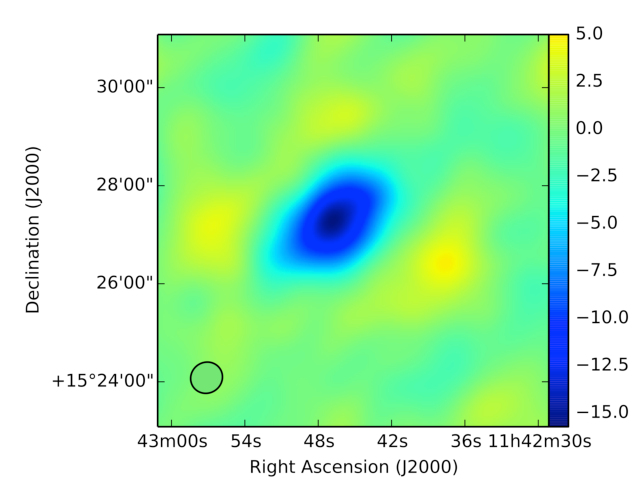
\includegraphics[width=0.35\textwidth]{./cluster.pdf}   
\hspace{0.1cm}
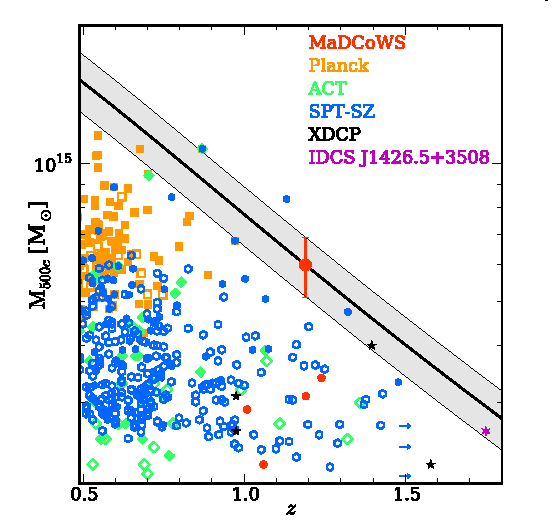
\includegraphics[width=0.28\textwidth]{./redshift_mass.pdf}
\hspace{0.2cm}  
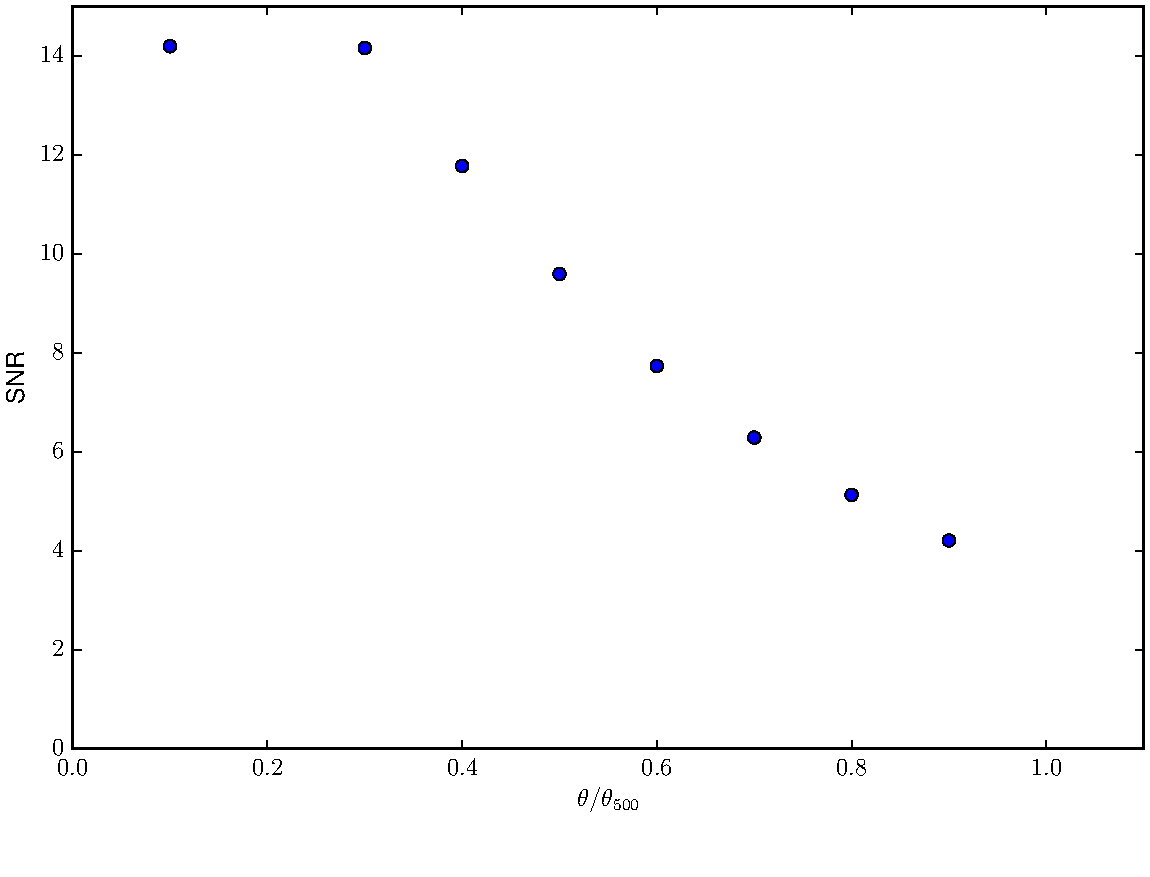
\includegraphics[width=0.33\textwidth]{./MOOJ1142_snr_prof.pdf}   
\caption{\footnotesize Left: CARMA SZ map of \moo\ covering a $8' \times 8'$ field in signal-to-noise unit. Middle: Comparison in the mass-redshift plane of \moo\ (large red circle with error bars) with other MaDCoWS clusters (red circles) and clusters from other surveys. Right: Expected signal-to-noise profile for a total observing time of 15 hours with NIKA2.}
\label{fig:SNRprof}
\end{figure}

\begin{thebibliography}{9}

\bibitem[Sif{\'o}n et al.(2016)]{sif16}
C. Sif{\'o}n, N. Battaglia,  M. Hasselfield, {\it et al.} (2016) MNRAS, \textbf{461}, 248-270

\bibitem[Pratt et al.(2009)]{pra09}
G.~W. Pratt, J.~H. Croston,  M. Arnaud, {\it et al.} (2009) A\&A, \textbf{498}, 361-378

\bibitem[Hoekstra et al.(2015)]{hoe15}
H. Hoekstra, R. Herbonnet,  A. Muzzin, {\it et al.} (2015) MNRAS, \textbf{449}, 685-714

\bibitem[Sunyaev \& Zeldovich(1972)]{sun72}
  R. A. Sunyaev, \& Y. B. Zel'dovich (1972), Astrophys. Space Phys. Res., \textbf{4}, 173
  
  \bibitem[Nagai et al.(2007)]{nag07}
  D. Nagai, A.~V. Kravtsov, A. Vikhlinin, {\it et al.} (2007), ApJ, \textbf{668}, 1-14
  
  \bibitem[Mantz et al.(2014)]{man14}
  A.~B. Mantz, S.~W. Allen, R.~G. Morris, {\it et al.} (2014), MNRAS, \textbf{440}, 2077
  
  \bibitem[Vikhlinin et al.(2009)]{vik09}
  A. Vikhlinin, A.~V. Kravtsov, R.~A. Burenin (2009), ApJ, \textbf{692}, 1060
  
  \bibitem[Sereno et al.(2015)]{ser15}
  M. Sereno, A. Veropalumbo, F. Marulli, {\it et al.} (2015), MNRAS, \textbf{449}, 4147
  
  \bibitem[Shandera et al.(2013)]{sha13}
  S. Shandera, A.~B. Mantz, B. Rapetti, {\it et al.} (2013), Cosmology~Astropart.~Phys., \textbf{8}, 4
  
  \bibitem[Adam et al.(2014)]{ada14}
R. Adam, B. Comis, J.-F. Mac\'ias-P\'erez, {\it et al.} (2014) A\&A, \textbf{569}, A66

\bibitem[Adam et al.(2015)]{ada15}
R. Adam, B. Comis, J.-F. Mac\'ias-P\'erez, {\it et al.} (2015) A\&A, \textbf{576}, A12

\bibitem[Adam et al.(2016)]{ada16a}
R. Adam, B. Comis, I. Bartalucci, {\it et al.} (2016) A\&A, \textbf{586}, A122

\bibitem[Adam et al.(2016)]{ada16b}
R. Adam, I. Bartalucci, G.W. Pratt, {\it et al.} (2016) arXiv:1606.07721

\bibitem[Ruppin et al.(2016)]{rup16}
F. Ruppin, R. Adam, B. Comis, {\it et al.} (2016) arXiv:1607.07679

\bibitem[Arnaud et al.(2010)]{arn10}
M. Arnaud, G.~W. Pratt, R. Piffaretti, {\it et al.} (2010) A\&A, \textbf{517}, A92

\bibitem[Sembolini et al.(2014)]{sem14}
  F. Sembolini, M. De Petris, G. Yepes, {\it et al.} (2014), MNRAS, \textbf{440}, 3520
  
\end{thebibliography}

\end{document}
